\documentclass{beamer}

\mode<presentation>


\usetheme{Madrid}

\usepackage{graphicx} % Allows including images
\usepackage{booktabs} % Allows the use of \toprule, \midrule and \bottomrule in tables
\usepackage{subcaption}
\usepackage[backend=biber,style=numeric]{biblatex}

\addbibresource{LPN.bib}

\title[LPN]{Learning Parity with Noise} % The short title appears at the bottom of every slide, the full title is only on the title page

\author{Botond Molnár} % Your name
\institute[University of Debrecen] % Your institution as it will appear on the bottom of every slide, may be shorthand to save space
{
University of Debrecen \\ % Your institution for the title page
\medskip
\textit{molnarbotond.eagle@gmail.com} % Your email address
}
\date{\today} % Date, can be changed to a custom date

\begin{document}

\begin{frame}
  \titlepage % Print the title page as the first slide
\end{frame}

\begin{frame}
  \frametitle{Overview} % Table of contents slide, comment this block out to remove it
  \tableofcontents % Throughout your presentation, if you choose to use \section{} and \subsection{} commands, these will automatically be printed on this slide as an overview of your presentation
\end{frame}

%------------------------------------------------
\section{The LPN Problem} % Sections can be created in order to organize your presentation into discrete blocks, all sections and subsections are automatically printed in the table of contents as an overview of the talk
%------------------------------------------------

\subsection{In General} % A subsection can be created just before a set of slides with a common theme to further break down your presentation into chunks

\begin{frame}
  \frametitle{The LPN Problem}
  \begin{figure}
    \centering
    \begin{subfigure}[b]{0.45\textwidth}
      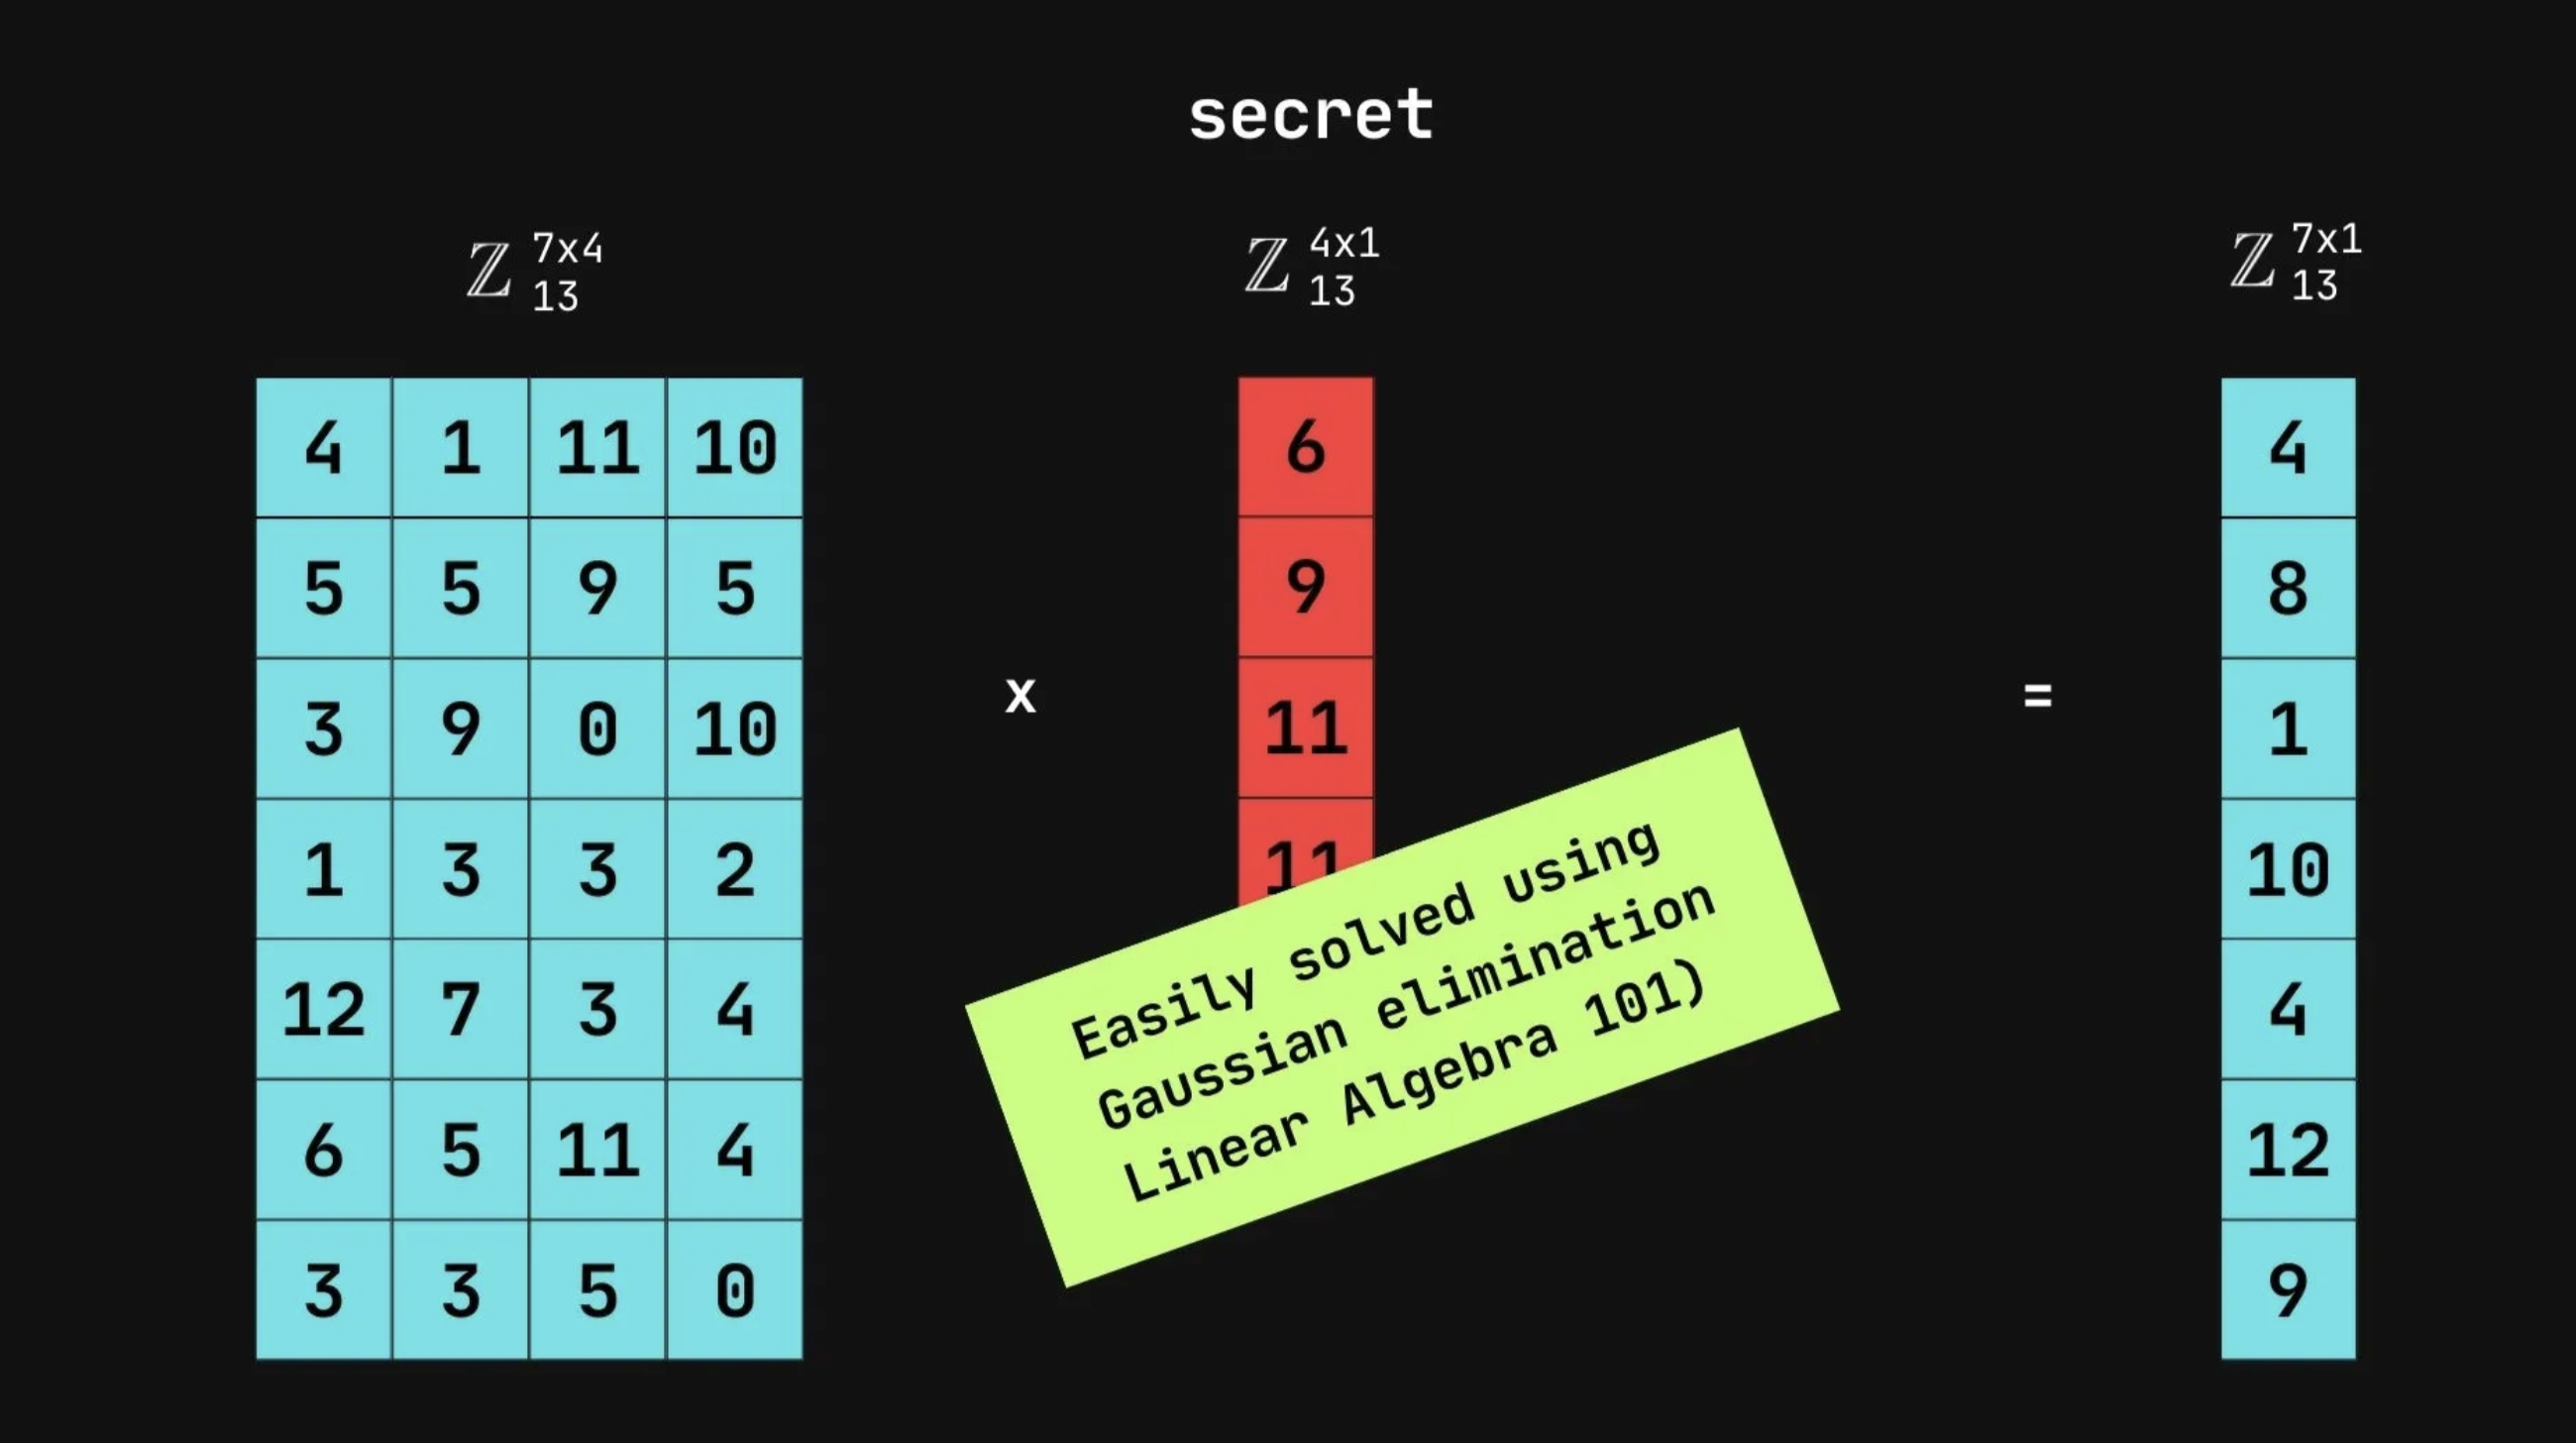
\includegraphics[width=1\textwidth]{lpn_preq.png}
      \caption{Matrix Multiplication}
      \label{fig:lpn_preq}
    \end{subfigure}
    \hfill
    \begin{subfigure}[b]{0.45\textwidth}
      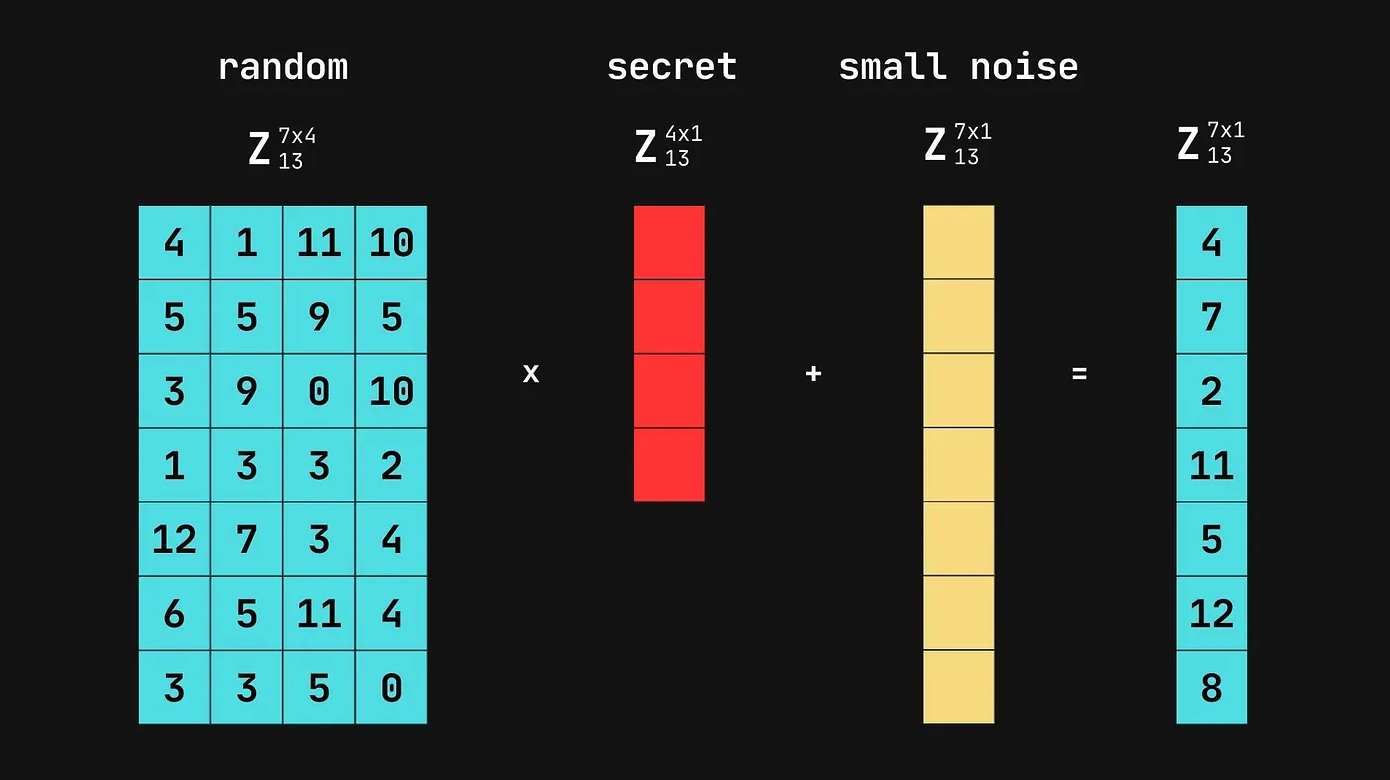
\includegraphics[width=1\textwidth]{lpn_problem.png}
      \caption{Add Noise}
      \label{fig:lpn_problem}
    \end{subfigure}
  \end{figure}
\end{frame}


\begin{frame}
  \frametitle{The LPN Problem}
  \begin{itemize}
    \item The LPN problem is a computational problem in the field of cryptography \cite{LPNluke2022medium}.
    \item It is a generalization of the Learning with Errors (LWE) problem.
    \item The problem is to find the secret key $s$ from the public key $A$ and the noisy output $b$.
    \item The public key $A$ is a matrix of size $m \times n$ and the secret key $s$ is a vector of size $n$.
    \item The noisy output $b$ is a vector of size $m$.
    \item The noise is added to the output by taking the dot product of the public key and the secret key and adding a vector of noise.
    \item It is a hard problem to find the secret key from the public key and the public parameters
  \end{itemize}
\end{frame}


\subsection{Formally}

\begin{frame}
  \frametitle{The LPN Problem}
  \begin{figure}
    \centering
    \caption{LPN Formally}
    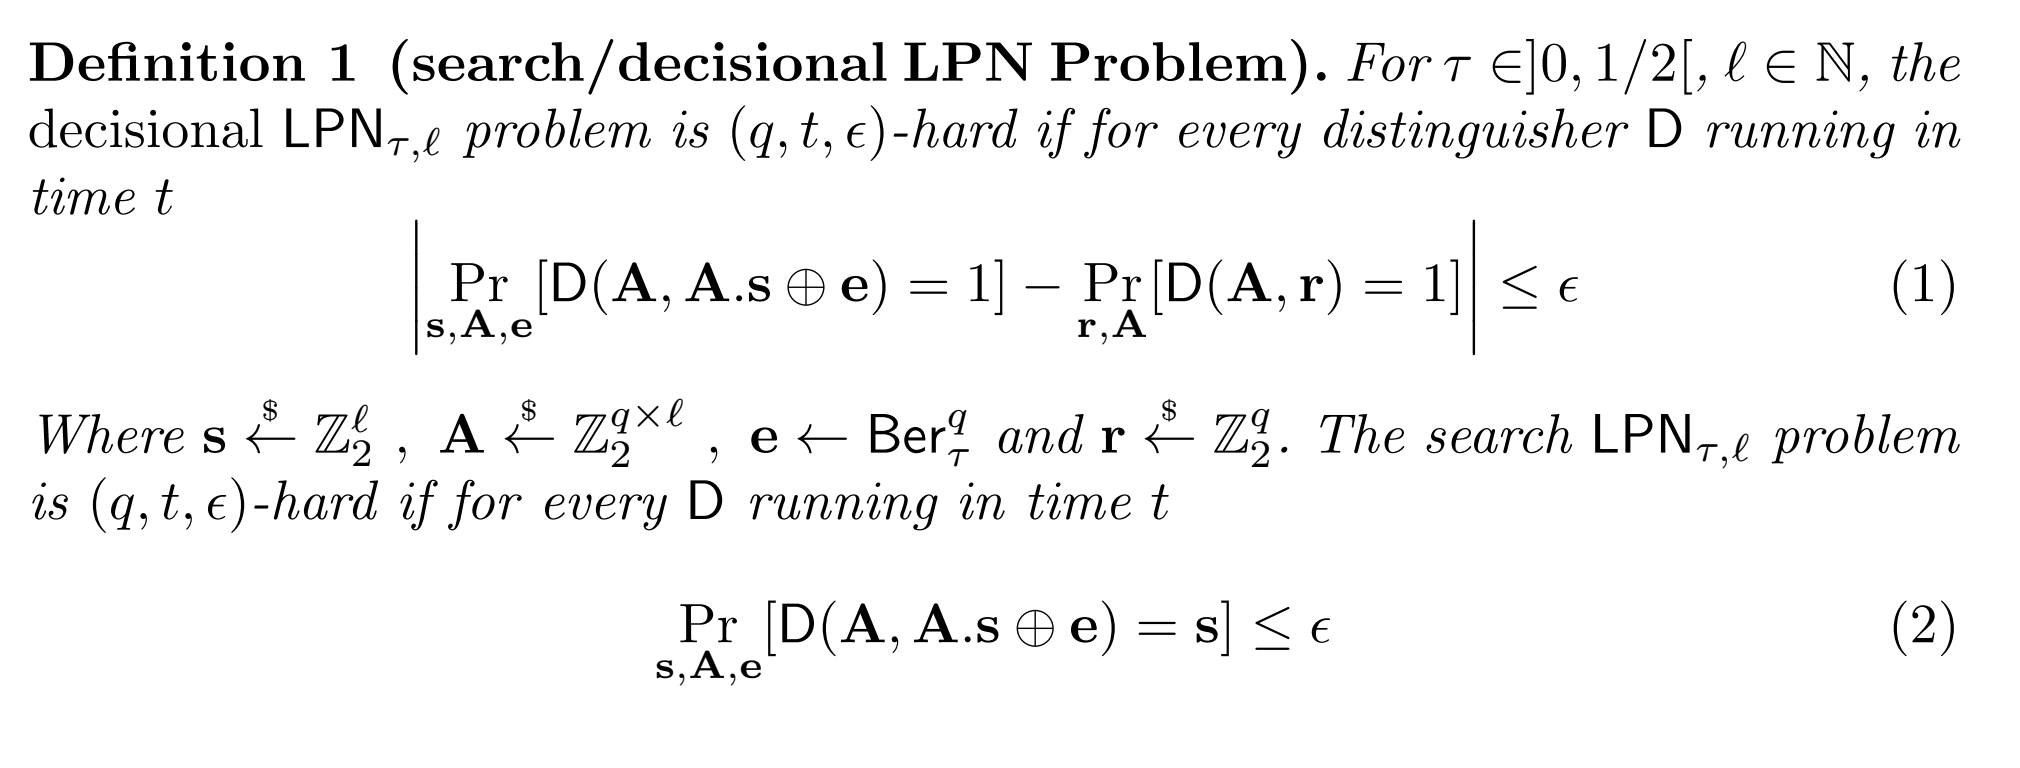
\includegraphics[width=0.9\textwidth]{lpn_problem_spec.png}
    \label{fig:lpn_problem_spec}
  \end{figure}
\end{frame}

\section{Public-key Encryption Scheme}

\begin{frame}{Public-key Encryption Scheme}
  \cite{base}'s encryption scheme is a improved version of \cite{damgard} scheme.
  \begin{itemize}
    \item Reducing the DLPN variety problem with $ S \leftarrow \textit{Ber}_r^{n \times n} $ to the normal DLPN problem.
    \item New single-bit public key encryption algorithm where the plaintext will be converted into a bit vector involved in cryptographic operations.
    \item The probability of the hamming weight exceeding expectations will exponentially decay rapidly to a value the is negligible.
    \item This ensures even if $r = 1/\sqrt{n}$ parameter is large the decription error can be ignored, therefore thr size of the public key is smaller than in \cite{damgard}'s scheme.
    \item Decryption and encryption time of the algorythm is greatly reduced.
    \item
  \end{itemize}
\end{frame}

\begin{frame}{Enrcrption Scheme}
  The scheme consists of three PPT algorithms:
  \begin{itemize}
    \item Key generation  $\rightarrow KeyGen(1^{\textit{n}}, r) $
    \item Enccryption  $\rightarrow Enc(pk, m) $
    \item Decryption  $\rightarrow Dec(sk, c) $
  \end{itemize}
\end{frame}

\begin{frame}{Key Generation}
  The key generation of the cryptosytem $ KeyGen(1^\mathbb{n}, r) $
  \begin{itemize}
    \item $ n $ integer
    \item $r$ noise rate
    \item Choose matrix $ A \leftarrow \mathbb{Z}_2^{n \times n} $ randomly
    \item Choose $ S \leftarrow Ber_r^{n \times n} $, $ E \leftarrow Ber_r^{n \times n} $
    \item Compute $ B = AS + E $
    \item Public key: $ pk = (A,B) $
    \item Secret key: $ sk = (S) $
  \end{itemize}
\end{frame}

\begin{frame}{Encryption}
  The encryption of the cryptosytem $ Enc(pk, m) $
  \begin{itemize}
    \item Input is $pk$ and $ m \in Z_2 $
    \item Compute $c_1 = r^T A + e_1^T, c_2 = r^T B + e^T_2$.
    \item Returns ciphertext $c = (c_1, c_2)$
  \end{itemize}
\end{frame}

\begin{frame}{Decryption}
  The decryption of the cryptosytem $ Dec(sk, c) $
  \begin{itemize}
    \item Input secret key $sk$ and ciphertext $c$
    \item Compute $ d = c_1 \times S + c_2 $
    \item If $ h(d) << n/2 $, It returns $m = 0$, else it return $m=1$
  \end{itemize}
\end{frame}

\begin{frame}{Comparison with RSA and Damgard's Scheme}
  \begin{itemize}
    \item It is faster than RSA
    \item It fells short of Damgard's scheme, while having the same public key size
    \item Decryption error is negligible.
    \item Not CCA secure, only IND-CPA secure.
  \end{itemize}
\end{frame}

\begin{frame}{Comparison}
  \begin{figure}
    \centering
    \caption{Comparison}
    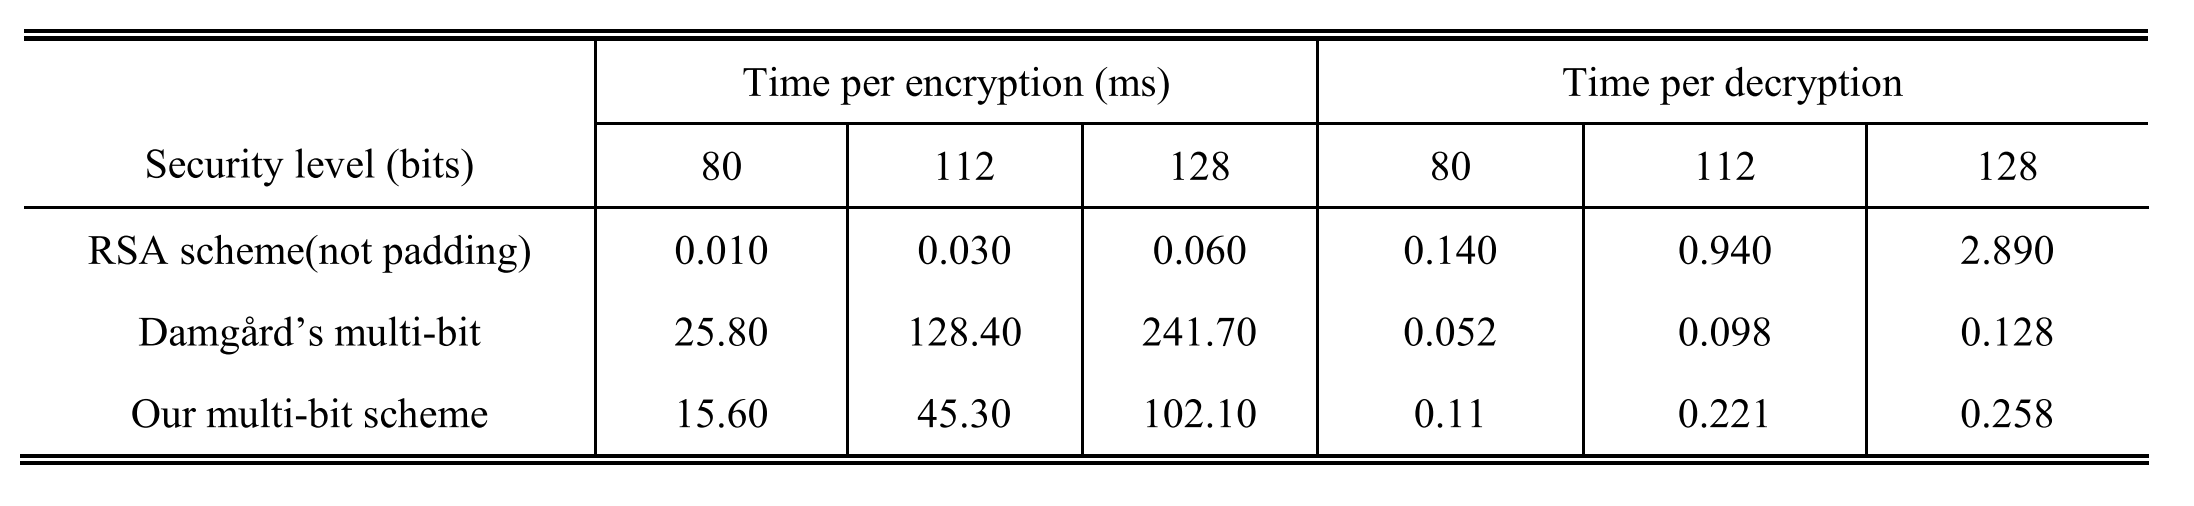
\includegraphics[width=0.9\textwidth]{comparison.png}
    \label{fig:comparison}
  \end{figure}
\end{frame}

\section{Future Research Aims}


\begin{frame}{Making the Scheme CCA Secure}
  \cite{CCA} extended the public key scheme to be IND-CCA1 and IND-CCA2 secure.
  To achieve IND-CCA1 security the author extended the scheme with an instance-key derivation step that assigns a tag to each ciphertext and derives an instance public or secret key for each the tag.
  These instance keys are used as keys for public key scheme.
  To achieve IND-CCA2 security the author introduced one-time signatures
\end{frame}

\section{Base IND-CPA PKE Scheme}

\begin{frame}{Base IND-CPA PKE Scheme Construction}
  \begin{itemize}
    \item Key generation: $KeyGen(1^k)$
    \item Encryption: $Enc(pk, m)$
    \item Decryption: $Dec(sk, c)$
    \item $k$ security parameter
    \item $n \in O(k^{2/(1-2 \epsilon )})$
    \item $ l_1, l_2, l_3 \in O(k^{2/(1-2 \epsilon)})$
    \item $ \rho = O(k^{-(1+2 \epsilon)/(1-2 \epsilon)}) $
    \item $G \in \mathbb{F}_2^{l_2 \times n}$ is the generator matrix of a binary linear error-correcting code $\mathcal{C}$
    \item $Decode_{\mathcal{C}}$ an efficient decoding procodeure for $\mathcal{C}$ that corrects up to $ \alpha l_2 $ errors ($\alpha$ is a constant)
    \item $ \mathcal{D} \subseteq \mathbb{F}^{l_3}_2 $ is a binary error correcting code with efficient encoding $Encode_{\mathcal{D}}$ and error-correction $Decode_{\mathcal{C}}$ which corrects up to $\lambda l_3$ errors

  \end{itemize}
\end{frame}

\begin{frame}{Base IND-CPA PKE Scheme Key Generation}
  $KeyGen(1^k)$:
  \begin{itemize}
    \item Sample matrix $ A \in \mathbb{F}_2^{l_1 \times n}$ uniformly at random.
    \item Sample matrix $ C \in \mathbb{F}_2^{l_3 \times n} $ uniformly at random.
    \item Sample the matrix $T$ from $ \mathcal{X}_p^{l_2 \times l_1} $
    \item Sample matrix $X$ from $\mathcal{X}_p^{l_2 \times n}$
    \item Set $B = G + T \cdot A + X$
    \item $pk = (A, B, C)$
    \item $sk = T$
  \end{itemize}
\end{frame}

\begin{frame}{Base IND-CPA PKE Scheme Encryption}
  $Enc_{pk}(m)$:
  \begin{itemize}
    \item Takes $pk = (A,B,C)$ and plaintext $m \in \mathbb{F}_2^n$
    \item Sample $s$ from $\mathcal{X}^n_{\rho}$, $e_1$ from $\mathcal{X}_{\rho}^{l_1}$, $e_2$ from $\mathcal{X}_{\rho}^{l_2}$,$e_3$ from $\mathcal{X}_{\rho}^{l_3}$
    \item Set $c_1  = A \cdot s + e_1, c_2 = B \cdot s + e_2, c_3 = C \cdot s + e_3 + Encode_{\mathcal{D}}(m)$
    \item Output $c = (c_1, c_2, c_3)$
  \end{itemize}
\end{frame}


\begin{frame}{Base IND-CPA PKE Scheme Decryption}
  $Dec_{sk}(c)$:
  \begin{itemize}
    \item Takes $sk = T$ and ciphertext $c = (c_1, c_2, c_3)$
    \item Computes $ y = c_2 - T \cdot c_1 $
    \item Runs error correcting $ s = Decode_{\mathcal{C}}(c_3 - C \cdot d ) $,  if succeeds run $ m = Decode_{\mathcal{D}}(c_3 - C \cdot s) $
    \item Outputs $m$
  \end{itemize}
\end{frame}

\begin{frame}{Correctness of the scheme}
  Decryption only fails if one of the two error decoding operations fails.
  Probability of faliure:
  \begin{itemize}
    \item It is sufficient to bound the hamming-weight of the error-term $ v = X \cdot s + e_2 - T \cdot e_1 $
    \item Fix constants $ \beta,\gamma > 0 $ such that $ 2\beta + \gamma \rho < \alpha $ and $ \gamma \rho < \lambda $
    \item By a Chernoff-bound it holds that $ |s| < \gamma \rho n, e_1 < \gamma \rho l_1, e_2 < \gamma \rho l_2, e_3 < \gamma \rho l_3 $ with owerwhelming probability $k$
    \item The decoding procedure can correct up to $\alpha l_2$ errors
    \item Altogether it holds that $$ |v| \leq |Xs| + |e_2| + |Te_1| \leq 2 \beta l_2 + \gamma \rho l_2 < \alpha l_2 $$
    \item Therefore, the decoding algorithm $Decode_{\mathcal{C}}$ will successfully recover $s$ and $Decode_{\mathcal{D}}$ will successfully recover $m$ as $$ |e_3| < \gamma \rho \cdot l_3 < \lambda l_3 $$
  \end{itemize}

\end{frame}

\begin{frame}{Expansion of the Base IND-CPA PKE Scheme}
  \cite{CCA} expanded the previous scheme with an instance-key derivation step  that assigns a tag to each ciphertext
  and derives a instance public or secret key for each the tag. These keys will be used as the keys for the PKE.

\end{frame}



\begin{frame}{IND-CCA1 Secure PKE Scheme Construction}
  \begin{itemize}
    \item $k$ security parameter
    \item $n \in O(k^{2/(1-2 \epsilon )})$
    \item $ l_1, l_2, l_3 \in O(k^{2/(1-2 \epsilon)})$
    \item $ \rho = O(k^{-(1+2 \epsilon)/(1-2 \epsilon)}) $
    \item $G \in \mathbb{F}_2^{l_2 \times n}$ is the generator matrix of a binary linear error-correcting code $\mathcal{C}$
    \item $Decode_{\mathcal{C}}$ an efficient decoding procodeure for $\mathcal{C}$ that corrects up to $ \alpha l_2 $ errors ($\alpha$ is a constant)
    \item $ \mathcal{D} \subseteq \mathbb{F}^{l_3}_2 $ is a binary error correcting code with efficient encoding $Encode_{\mathcal{D}}$ and error-correction $Decode_{\mathcal{C}}$ which corrects up to $\lambda l_3$ errors
    \item $\mathcal{E} \in \Sigma^{l_2} $ be a q-ary code over alphabet $\Sigma$ ($q = |\Sigma|$) with relative minimum-distance $\delta$ and dimension $n$
    \item It is sufficient to choose $\delta < 1-1/q$ such that $2\beta + \gamma \rho + 1 - \delta < \alpha$, since $\alpha$ must be big enough to correct the decryption error which has a hamming weight $\leq (2\beta + \gamma \rho)l_2, \beta > 0$ and the additional error included by erasures will have a hamming weight $ \leq (1-\delta)l_2$
  \end{itemize}

\end{frame}

\section{IND-CCA1 Secure PKE Scheme}

\begin{frame}{IND-CCA1 Secure PKE Scheme Construction}
  \begin{itemize}
    \item Since $\beta$ and $\gamma$ can be chosen arbitrarily small, we can always find $q$ and $\delta$ such that the requirements are met.
    \item Therefore, fix $\beta, \gamma, q, \delta$ so that dor sufficiently large $n$ it holds that
          $$ 2\beta + \delta \rho + 1 - \delta < \alpha $$
  \end{itemize}
\end{frame}


\begin{frame}{IND-CCA1 Secure PKE Scheme Key Generation}
  $KeyGen(1^k)$:
  \begin{itemize}
    \item Sample matrix $A \in \mathbb{F}_2^{l_1 \times n}$ uniformly at random
    \item Sample matrix $ C \in \mathbb{F}^{l_3 \times n}_2$ uniformly at random
    \item For every $j \in \Sigma$ sample a matrix $T_j$ from $\mathcal{X}_{\rho}^{l_2 \times l_1}$ and matrix $X_j$ from $\mathcal{X}_{\rho}^{l_2 \times n}$
    \item Set $B_j = G + T_j \cdot A + X_j$
    \item Set $pk = (A, (B_j)_{j \in \Sigma}, C)$
    \item Set $sk = (T_j)_{j \in \Sigma}$
  \end{itemize}
\end{frame}

\begin{frame}{IND-CCA1 Secure PKE Scheme Encryption}
  $Enc_{pk}(m)$:
  \begin{itemize}
    \item Takes $pk = (A, (B_j)_{j \in \Sigma}, C)$ and plaintext $m \in \mathbb{F}^n_2$
    \item Write each $B_j$ as $B_j = (b_{j,1},...,b_{j, l_2})^T$
    \item Smaple a tag $\tau \in \Sigma^n$ uniformly at random and set $\hat{\tau} = Encode_{\mathcal{E}}(\tau)$
    \item Set $B_{\hat{\tau}} = (b_{\hat{\tau}, 1}, ... ,b_{\hat{\tau}_{l_2}, l_2})^T$
    \item Encryption samples $s$ from $\mathcal{X}_{\rho}^{l_1}$, $e_1$ from $\mathcal{X}_{\rho}^{l_1}$, $e_2$ from $\mathcal{X}_{\rho}^{l_2}$, $e_3$ from $\mathcal{X}_{\rho}^{l_3}$
    \item Set $c_1 = A \cdot s + e_1, c_2 = B_{\hat{\tau}} \cdot s + e_2, c_3 = C \cdot s + e_3 + Encode_{\mathcal{D}}(m)$
    \item Output $c = (c_1, c_2, c_3, \tau)$
  \end{itemize}
\end{frame}

\begin{frame}{IND-CCA1 Secure PKE Scheme Decryption}
  $Dec_{sk}(c)$:
  \begin{itemize}
    \item Takes $sk = (T_j)_{j \in \Sigma}$ and ciphertext $c = (c_1, c_2, c_3, \tau)$
    \item Write each $T_j$ as $T_j = (t_{j,1},...,t_{j, l_2})^T$
    \item Compute $\hat{\tau} = Encode_{\mathcal{E}}$ and $T_{\hat{\tau}} = (t_{\hat{\tau}, 1}, ... , )$
    \item Compute $y = c_2 - T_{\hat{\tau}} \cdot c_1$ and $s = Decode_{\mathcal{C}}(y)$
    \item Outputs nil if the decoding fails, else computes $m = Decode_{\mathcal{D}}(c_3 - C \cdot s)$
    \item Computes $e_1 = c_1 -A \cdot s, e_2 = c_2 -B_{\hat{\tau}} \cdot s, e_3 = c_3 - C \cdot s - Encode_{\mathcal{D}}(m)$
    \item Checks if $|s| < \gamma \rho n$, $|e_1| < \gamma \rho l_1$, $|e_2| < \gamma \rho l_2$, $|e_3| < \gamma \rho l_3$
    \item If all coditions met outputs $m$, else outputs nil.
  \end{itemize}
\end{frame}

\begin{frame}{Correctness of the IND-CCA1 Secure PKE Scheme}
  Correcness can be derived from the previous scheme with the only additional step of checking the hamming weights $|s|, |e_1|, |e_2|, |e_3|$
\end{frame}

\begin{frame}{Room for Improvement}
  \begin{itemize}
    \item The scheme is IND-CCA1 secure, but not IND-CCA2 secure
    \item \cite{CCA} extended the scheme to be IND-CCA2 secure by introducing one-time signatures
  \end{itemize}
\end{frame}

\section{IND-CCA2 Secure PKE Scheme}

\begin{frame}{Observations}
  \begin{itemize}
    \item The previous CCA1 secure scheme can be improved to be CCA2 secure.
    \item The scheme can be extended with one-time signatures to achieve CCA2 security.
    \item \cite{CCA} mentions that it is not necessary to choose tag $\tau \in \Sigma^n$ uniformly at random in the ecryption procedure of the prevous PKE scheme.
    \item The scheme must only guarantee that a PPT adversary $\mathcal{A}$ will have a negligible probablity of guessing the secret tag $\tau^*$ correctly if it is granted a polynomial number of trials.
    \item Therefore it is sufficient to sample the tags $\tau$ from a distribution with high min-entorpy.
  \end{itemize}

\end{frame}

\begin{frame}{IND-CCA2 Secure PKE Scheme Construction}
  \begin{itemize}
    \item $SIG = (Gen, Sign, Verify)$ be an EUF-CMA secure one time signature scheme.
    \item Key generation is identical to the previous CCA1 secure scheme
    \item Enc first computes a pair of verification keys a pair of verification and signture-keys $(vk, sk) = SIG.Gen(1^k)$
    \item Then it runs the encryption procedure of the previous scheme $PKE.Enc$.
    \item The only difference that it sets $\tau = vk$ instead of choosing $\tau$ uniformly at random.
  \end{itemize}
\end{frame}

\begin{frame}{IND-CCA2 Secure PKE keygen}
  $KeyGen(1^k)$:
  The same as the previous CCA1 secure scheme
\end{frame}

\begin{frame}{IND-CCA2 Secure PKE Encryption}
  $Enc_{pk}(m)$:
  \begin{itemize}
    \item Generate $(vk, sgk) = SIG.Gen(1^k)$
    \item Encrypt $c' = Enc_{pk}'(m, vk)$
    \item Sign $\sigma = SIG.Sign_{sgk}(c')$, output $c = (c'. \sigma)$
  \end{itemize}

\end{frame}

\begin{frame}{IND-CCA2 Secure PKE Decryption}
  $Dec_{sk}(c)$:
  \begin{itemize}
    \item $c = (c', \sigma), c' = (\tau, c_1, c_2, c_3)$
    \item Set $vk = \tau$
    \item Check if $SIG.Verify_{vk}(c', \sigma) = 1$, if not abort
    \item Compute $m = PKE.Dec_{sk}(c')$
  \end{itemize}

\end{frame}

\begin{frame}{Proving IND-CCA2 Security}
  If $SIG$ is an EUF-CMA secure one-time signature scheme and the security level of the previous PKE scheme stands the scheme is IND-CCA2 secure.
\end{frame}

\section{Aim of Our Research}

\begin{frame}{Aim of Our Research}
  Our research goal is to make \cite{base}'s public key encryption scheme IND-CCA2 secure, and to integrate it into a lightwegiht adhoc mixnet
  which can be used in a drone network prividing anonymity and confidentiality.
  We turned for inspiration to \cite{CCA} to achieve IND-CCA2 in \cite{base}'s cryptosystem.
\end{frame}

\begin{frame}{}
  \centering Thanks for your attention!
\end{frame}

\begin{frame}{References}
  \printbibliography[title=References, heading=bibnumbered,resetnumbers=true]
\end{frame}


\end{document}
